\documentclass[t]{beamer}
\usetheme{Copenhagen}
\setbeamertemplate{headline}{} % remove toc from headers
\beamertemplatenavigationsymbolsempty

\usepackage{amsmath, array, tikz, bm, pgfplots, tcolorbox, tkz-euclide}
\usetkzobj{all}
\pgfplotsset{compat = 1.16}

\title{Exploring Angle Pairs}
\author{}
\date{}

% \begin{tcolorbox}[colframe=green!20!black, colback = green!30!white,title=\textbf{TITLE}]

\AtBeginSection[]
{
  \begin{frame}
    \frametitle{Objectives}
    \tableofcontents[currentsection]
  \end{frame}
}

\begin{document}

\begin{frame} 
\maketitle
\end{frame}

\begin{frame}{Adjacent Angles}
Two angles are adjacent if they
\begin{itemize}
	\item Share a common side
	\onslide<2->{\item Share a common vertex}
	\onslide<3->{\item Have no common interior points}
\end{itemize}
\vspace{8pt}
\begin{minipage}{0.35\textwidth}
\begin{center}
\begin{tikzpicture}
\tkzDefPoints{0/0/A, 2/-0.5/B}
\tkzDefShiftPoint[A](90:2.25){C}
\tkzDefShiftPoint[A](40:2.25){D}
\tkzDrawSegments[->, >=stealth](A,C A,B A,D)
\tkzLabelAngle[pos=0.75](B,A,D){1}
\tkzLabelAngle[pos=0.75](C,A,D){2}
\end{tikzpicture}
\end{center}
\end{minipage}
\begin{minipage}{0.6\textwidth}
\onslide<4->{$\angle 1 \text{ and } \angle 2$ are adjacent angles.}
\end{minipage}
\end{frame}

\begin{frame}{Vertical Angles}
Vertical angles are formed by 2 intersecting lines.	\newline\\
\begin{center}
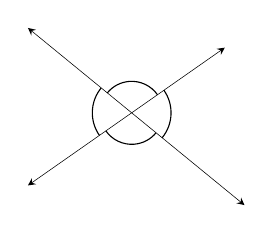
\begin{tikzpicture}
\tkzDefPoints{0/0/A, 2.5/1.75/B, 0/2/C, 2.75/-0.25/D}
\tkzDrawSegments[<->,>=stealth](A,B C,D)
\tkzInterLL(A,B)(C,D) \tkzGetPoint{E}
\tkzMarkAngles[size=0.5,fill=red!60](C,E,A D,E,B)
\tkzMarkAngles[size=0.4,fill=blue!60](B,E,C A,E,D)
\end{tikzpicture}
\end{center}
\end{frame}

\begin{frame}{Complementary Angles}
\begin{tcolorbox}[colframe=green!20!black, colback = green!30!white,title=\textbf{Complementary Angles}]
Two or more angles that add up to $90^\circ$
\end{tcolorbox}
\vspace{8pt}	\pause
\begin{center}
\begin{tikzpicture}
\tkzDefPoints{0/0/A, 2/-0.4/B, 4/0/D, 6/0/E}
\tkzDefShiftPoint[A](53:2){C}
\tkzDefShiftPoint[D](37:2){F}
\tkzDrawSegments[->,>=stealth](A,B A,C D,E D,F)
\tkzLabelAngle[pos=0.75](B,A,C){$53^\circ$}
\tkzLabelAngle[pos=0.85](E,D,F){$37^\circ$}
\end{tikzpicture}
\end{center}
\end{frame}

\begin{frame}{Supplementary Angles}
\begin{tcolorbox}[colframe=green!20!black, colback = green!30!white,title=\textbf{Supplementary Angles}]
Two or more angles that add up to $180^\circ$
\end{tcolorbox}
\vspace{8pt}	\pause
\begin{center}
\begin{tikzpicture}
\tkzDefPoints{0/0/A, 2/-0.4/B, 4/0/D, 6/0/E}
\tkzDefShiftPoint[A](110:2){C}
\tkzDefShiftPoint[D](70:2){F}
\tkzDrawSegments[->,>=stealth](A,B A,C D,E D,F)
\tkzLabelAngle[pos=0.75](B,A,C){$110^\circ$}
\tkzLabelAngle[pos=0.85](E,D,F){$70^\circ$}
\end{tikzpicture}
\end{center}
\end{frame}

\tikzset{
	ex1/.pic={
		\tkzDefPoints{0/0/F, 2/0/C}
    	\tkzDefShiftPoint[F](28:2){B}
    	\tkzDefShiftPoint[F](118:2){A}
    	\tkzDefShiftPoint[F](180:2){E}
    	\tkzDefShiftPoint[F](-62:2){D}
    	\tkzDrawSegments[add = 0 and 0.25, ->, >=stealth](F,A F,B F,C F,D F,E)
    	\tkzLabelPoints[below](C,E)
    	\tkzLabelPoints[right](A,D)
    	\tkzLabelPoints[below right](F)
    	\tkzLabelPoints[above](B)
    	\tkzDrawPoints(A,B,C,D,E)
    	\tkzLabelAngle(C,F,B){$28^\circ$}
    	\tkzLabelAngle[pos=0.6](A,F,E){$62^\circ$}
    	\tkzLabelAngle[pos=-0.5](E,F,D){$118^\circ$}
	}
}
\begin{frame}{Example 1}
Use the diagram to determine if each statement is true.
\begin{center}
\tikz \pic[scale=0.8]{ex1};
\end{center}
(a) \quad $\angle BFD$ and $\angle AFB$ are adjacent angles. 	\quad \onslide<2->{True}   \newline\\
\onslide<3->{(b) \quad $\angle AFB$ and $\angle EFD$ are vertical angles.}	\quad \onslide<4->{False}    \newline\\
\onslide<5->{(c) \quad $\angle AFE$ and $\angle BFC$ are complementary.}		\quad \onslide<6->{True}
\end{frame}

\begin{frame}{Angle Bisectors}
An \textbf{angle bisector} is a ray (or segment) that divides an angle into 2 congruent angles.
\begin{center}
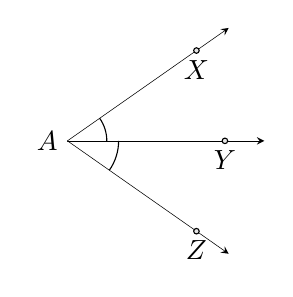
\begin{tikzpicture}
    \tkzDefPoints{0/0/A, 2/0/Y}
    \tkzDefShiftPoint[A](35:2){X}
    \tkzDefShiftPoint[A](-35:2){Z}
    \tkzDrawSegments[->, >=stealth, add = 0 and 0.25](A,X A,Z A,Y)
    \tkzDrawPoints(X,Y,Z)
    \tkzLabelPoints[below](X,Y,Z)
    \tkzLabelPoints[left](A)
    \tkzMarkAngle[size=0.5](Y,A,X)
    \tkzMarkAngle[size=0.65](Z,A,Y)
\end{tikzpicture}
\end{center}
\vspace{8pt}

\onslide<2->{\[\overrightarrow{AY} \text{ bisects } \angle XAZ \onslide<3->{\longrightarrow \angle XAY \cong \angle ZAY\]}}
\end{frame}

\begin{frame}{Example 2}
(a)	\quad $\overrightarrow{AC}$ bisects $\angle DAB$. What is $m\angle DAB$?
\begin{center}
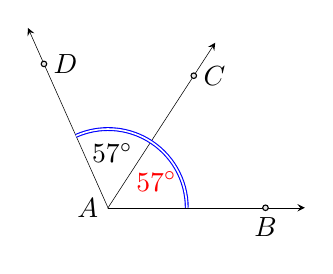
\begin{tikzpicture}
\tkzDefPoints{0/0/A, 2/0/B}
\tkzDefShiftPoint[A](57:2){C}
\tkzDefShiftPoint[A](114:2){D}
\tkzDrawSegments[add = 0 and 0.25, ->, >=stealth](A,B A,C A,D)
\tkzDrawPoints(B,C,D)
\tkzLabelPoints[right](D,C)
\tkzLabelPoints[left](A)
\tkzLabelPoints[below](B)
\tkzLabelAngle[pos=0.7](C,A,D){$57^\circ$}
\onslide<2->{\tkzLabelAngle[pos=0.7](B,A,C){\color{red}$57^\circ$}}
\onslide<3->{\tkzMarkAngle[color=blue,double,pos=1.5](B,A,D)}
\end{tikzpicture}
\end{center}
\onslide<4->{\[m\angle DAB = 114^\circ\]}
\end{frame}

\begin{frame}{Example 2}
(b)	\quad $\overrightarrow{KM}$ bisects $\angle JKL$. If $m\angle JKL = 72^\circ$, what is $m\angle JKM$?
\onslide<2->{
	\begin{center}
	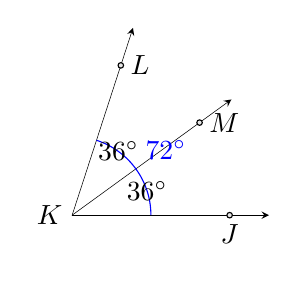
\begin{tikzpicture}
	\tkzDefPoints{0/0/K, 2/0/J}
	\tkzDefShiftPoint[K](36:2){M}
	\tkzDefShiftPoint[K](72:2){L}
	\tkzDrawSegments[add = 0 and 0.25, ->, >=stealth](K,J K,L K,M)
	\tkzDrawPoints(J,M,L)
	\tkzLabelPoints[right](L,M)
	\tkzLabelPoints[left](K)
	\tkzLabelPoints[below](J)
	\tkzMarkAngle[color=blue](J,K,L)
	\tkzLabelAngle[color=blue,above right](J,K,L){$72^\circ$}
	\onslide<3->{\tkzLabelAngle(J,K,M){$36^\circ$}}
	\onslide<3->{\tkzLabelAngle(M,K,L){$36^\circ$}}
	\end{tikzpicture}
	\end{center}
}
\onslide<4->{\[m\angle JKM = 36^\circ\]}
\end{frame}

\begin{frame}{Example 2}
(c)	\quad In the diagram, $RQ$ bisects $angle PRS$. Find the value of $x$.	\newline\\

\begin{minipage}{0.4\textwidth}
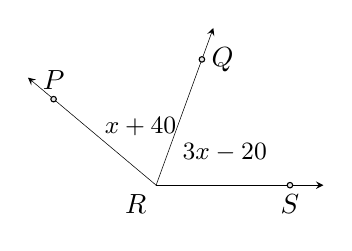
\begin{tikzpicture}[scale=0.85]
    \tkzDefPoints{0/0/R, 2/0/S}
    \tkzDefShiftPoint[R](70:2){Q}
    \tkzDefShiftPoint[R](140:2){P}
    \tkzDrawSegments[add = 0 and 0.25, ->, >=stealth](R,S R,P R,Q)
    \tkzDrawPoints(P,Q,S)
    \tkzLabelPoints[above](P)
    \tkzLabelPoints[right](Q)
    \tkzLabelPoints[below](S)
    \tkzLabelPoints[below left](R)
    \tkzLabelAngle[pos=0.9](Q,R,P){\small $x+40$}
    \node at (0.25,0.2) [anchor = south west] {\small $3x-20$};
\end{tikzpicture}
\end{minipage}
\begin{minipage}{0.55\textwidth}
\begin{align*}
\onslide<2->{x+40 &= 3x-20} \\
\onslide<3->{40 &= 2x - 20} \\
\onslide<4->{60 &= 2x} \\
\onslide<5->{x &= 30} \\
\end{align*}
\end{minipage}
\vspace{12pt}
\onslide<6->{Check:}
\begin{align*}
\onslide<7->{30 + 40 &\stackrel{?}{=} 3(30) - 20?} \\
\onslide<8->{70 &= 70}
\end{align*}
\end{frame}

\begin{frame}{Linear Pairs}
\begin{tcolorbox}[colframe=green!20!black, colback = green!30!white,title=\textbf{Linear Pair}]
A \textbf{linear pair} are two adjacent angles whose non-common sides form a line.
\end{tcolorbox}
\vspace{8pt}	\pause
\begin{center}
\begin{tikzpicture}
\tkzDefPoints{0/0/A, 4/0/B, 2.25/0/C, 3/1.75/D}
\tkzDrawSegment[<->,>=stealth](A,B)
\tkzDrawSegment[->,>=stealth](C,D)
\tkzLabelAngle[pos=0.35](D,C,A){1}
\tkzLabelAngle[pos=0.5](B,C,D){2}
\end{tikzpicture}
\end{center}
\onslide<3->{Angles 1 and 2 form a linear pair.}	\newline\\
\onslide<4->{$m\angle 1 + m\angle 2 = 180^\circ$}
\end{frame}

\begin{frame}{Example 3}
(a) \quad Find the $m\angle KPL$ and $m\angle JPL$ in the diagram.
\newline\\
\begin{center}
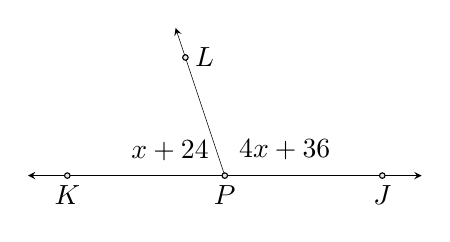
\begin{tikzpicture}
    \tkzDefPoints{0/0/K, 2/0/P, 4/0/J, 1.5/1.5/L}
    \tkzDrawSegments[add = 0 and 0.25, ->, >=stealth](P,K P,J P,L)
    \tkzDrawPoints(K,P,J,L)
    \tkzLabelPoints[below](K,P,J)
    \tkzLabelPoints[right](L)
    \tkzLabelAngle[pos=0.1, above left](L,P,K){$x+24$}
    \tkzLabelAngle[pos=0.1, above right](J,P,L){$4x+36$}
\end{tikzpicture}
\end{center}
\begin{align*}
	\onslide<2->{x+24 + 4x+36 &= 180} \\
	\onslide<3->{5x+60 &= 180} \\
	\onslide<4->{5x &= 120} \\
	\onslide<5->{x &= 24}
\end{align*}
\end{frame}

\begin{frame}{Example 3a \quad $x = 24$}
\begin{center}
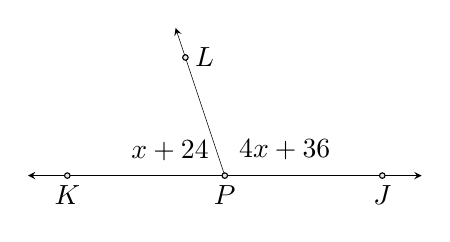
\begin{tikzpicture}
    \tkzDefPoints{0/0/K, 2/0/P, 4/0/J, 1.5/1.5/L}
    \tkzDrawSegments[add = 0 and 0.25, ->, >=stealth](P,K P,J P,L)
    \tkzDrawPoints(K,P,J,L)
    \tkzLabelPoints[below](K,P,J)
    \tkzLabelPoints[right](L)
    \tkzLabelAngle[pos=0.1, above left](L,P,K){$x+24$}
    \tkzLabelAngle[pos=0.1, above right](J,P,L){$4x+36$}
\end{tikzpicture}
\end{center}
\begin{align*}
\onslide<2->{m\angle KPL &= 24+24 & m\angle JPL &= 4(24)+36}	\\
\onslide<3->{m\angle KPL &= 48^\circ & m\angle JPL &= 132^\circ}
\end{align*}
\end{frame}

\end{document}